\chapter[Numerical and Experimental Methodologies]{Numerical and Experimental Methodologies}{Numerical and Experimental Methodologies}\label{CH4:NEM}

\section{Introduction}
The numerical simulations in this study were performed using ANSYS Fluent 2021 R1, a commercially available Computational Fluid Dynamics (CFD) software. The combustor geometry was spatially discretized with structured mesh using ICEM CFD 2021 R1. The main objectives of these simulations were to investigate the flow field, recirculation ratio and the temperature distribution in order to complement the experimental measurement for detailed understating. Both reacting and non-reacting flows were simulated, with a fixed equivalence ratio ($\phi$) of 0.8. It is important to note that a consistent 6.25 kW heat load was maintained across all cases. By conducting these numerical simulations under the given operating conditions, a comprehensive understanding of the flow characteristics, temperature profiles, and recirculation patterns can be obtained.

\section{\textbf{Numerical setup}}
\subsection{Combustor Mesh}
In order to simulate the combustor, a three-dimensional geometric model is constructed and meshing is done with using ICEM CFD software. Meshes for both the combustors are shown in figure \ref{Mesh}. Individual boundaries has been assigned names such as ``AIR INLET" and ``FUEL INLET" for inlets, ``EXIT" for exhaust, ``AIR WALL", ``FUEL TUBE" and ``EXIT WALL" for walls and ``SYMM" is assigned to symmetry plane. Only half of the flow domain is discretized into computational domain to reduce the associated computational cost. A total of $\approx$ 0.7 million hex-hedral structured mesh is created. At circular cross-sections ``C-Grid" is created to improve the mesh orthogonality with minium global quality index of of 68$\%$ and maximum aspect ratio of $\approx$ 63. 

\begin{figure}[!ht]
    \centering
	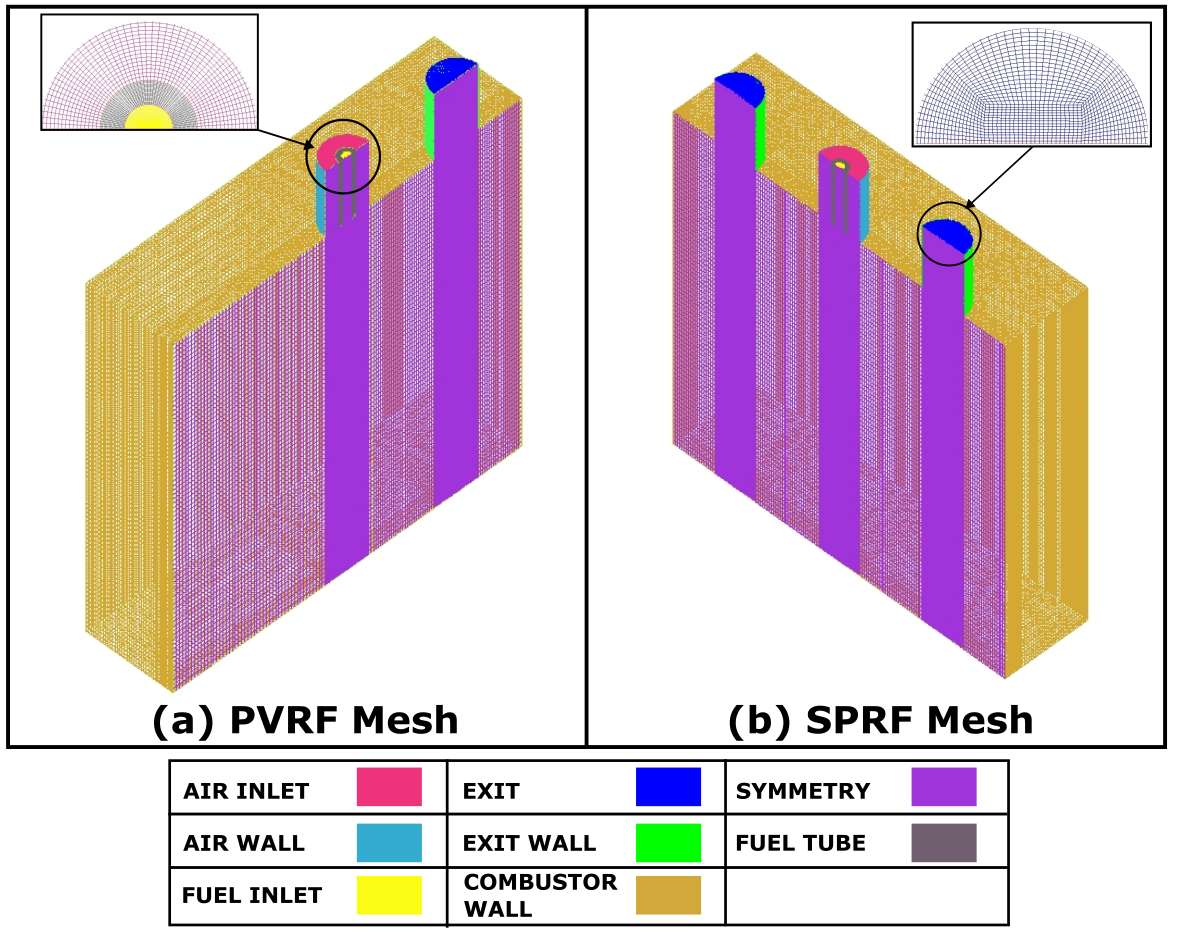
\includegraphics[width=0.9\textwidth]{Chapter4/Images/Mesh.png}
	\caption{Numerical mesh generated for the both combustor (PVRF, SPRF)}
	\label{Mesh}
\end{figure}

\subsection{Initial and Boundary Conditions}
The mass flow inlet boundary condition with  air mass flow rate ($\dot{m}_{air}$) 2.68 g/s and fuel mass flow rate ($\dot{m}_{fuel}$) 0.125 g/s with O$_2$ (0.21) and CH$_4$ (1) species mole fraction  is applied to the air and fuel inlets, respectively.
Pressure outlet boundary condition with zero gauge pressure (in Pa) and O$_2$ (0.21) mole fraction is applied to outlet (exit) of the combustor.
For walls, no-slip, stationary wall and standard wall roughness with 0.5 roughness constant, adiabatic, non-catalytic and zero diffusive flux for species boundary conditions are applied.
Symmetry boundary condition is applied at symmetry plane along which the combustor is cut into half. The operating pressure is 1 atm for all the cases and the initial temperature at the inlet and outlet is 300 K.

\subsection{Turbulence and Combustion Model}
SIMPLE scheme is used for coupling between pressure and velocity in the context of finite volume formulation. Second-order upwind schemes are used to discretize momentum and energy equations, while first-order upwind schemes are employed for other scalar quantities. To solve governing equations, a pressure-based solver is used. Gradients within the computational domain are computed using the least square cell-based method. Turbulence intensity of the mean velocity field is set at 5$\%$ with associated hydraulic diameter of 10 mm.

The standard k-$\epsilon$ model, combined with standard wall functions, is employed for turbulence modeling. This model, consisting of two transport equations to captures the diffusion of turbulent energy and convection. In particular, the turbulent kinetic energy (k), reflecting the energy within turbulence, and the turbulent dissipation rate ($\epsilon$), governing the rate at which k dissipates.

% \begin{equation}
%     \frac{\partial}{\partial t}(\rho k) \ + \ \frac{\partial}{\partial x_i}(\rho k u_i) \ =  \ \frac{\partial}{\partial x_j} \left[ \left( \mu + \frac{\mu_t}{\sigma_k} \right)\frac{\partial k}{\partial x_j} \right]\ +\ P_k \ + \ P_b \ - \ \rho\epsilon \ + \ S_k
% \end{equation}

% \begin{equation}
%     \frac{\partial}{\partial t}(\rho \epsilon) \ + \ \frac{\partial}{\partial x_i}(\rho \epsilon u_i) \ =  \ \frac{\partial}{\partial x_j} \left[ \left( \mu + \frac{\mu_t}{\sigma_{\epsilon}} \right)\frac{\partial \epsilon}{\partial x_j} \right]\ + \ C_{1\epsilon} \frac{\epsilon}{k} P_k  \ - \ C_{2\epsilon}\rho \frac{\epsilon^2}{k}  \ + \ S_{\epsilon}
% \end{equation}
% where 
% $$\mu_t = \rho C_{\mu}\frac{k^2}{\epsilon}, \
%     P_k = -\rho \overline{u_i^{'} u_j^{'}}\frac{\partial u_j}{\partial x_i}  \ = \ \mu_t S^2, \
%     S \ = \ \sqrt{2S_{ij}S_{ij}}, \ P_b \ = \ \beta g_i \frac{\mu_t}{Pr_t}\frac{\partial T}{\partial x_i}, \ \beta \ = \ -\frac{1}{\rho}\left( \frac{\partial \rho}{\partial T} \right)_p
% $$
% with model constants
% $$
% C_{1\epsilon} \ = \ 1.44, \ C_{2\epsilon} \ = \ 1.92, \ C_{\mu} \ = \ 0.09, \ \sigma_k \ = \ 1.0, \ \sigma_{\epsilon} \ = \ 1.3
% $$
 
The turbulence-chemistry interactions are accounted by using Eddy Dissipation Concept Model (EDCM), along with a two-step global reaction mechanism with volume fraction constant of 2.137 and time scale constant of 0.41. For mixture of reactants, incompressible ideal gas option is used to calculate density, mixing law is used for specific heat (Cp) calculation. Thermal conductivity is set constant 1.72$\times$10$^{-5}$ and mass diffusivity is set 2.88$\times$10 $^{-5}$ using constant-dilute approximation.

% Reactions involved in two step methane-air mechanism are as follows:
% $$
% CH_4 + 1.5\ O_2 \rightarrow CO_2 + 2 \ H_2O
% $$
% $$
% CO + 0.5 \ O_2 \rightarrow CO_2
% $$
% $$
% CO_2 \rightarrow CO + 0.5 \ O_2
% $$

Table \ref{Numerical Model} provides a concise overview of the numerical model parameters, encompassing the essential specifications and configurations employed in the simulation.

\begin{table}[h!]
\centering
\caption{Numerical model specification}
\begin{tabular}{|l| m{8cm}| }
\hline
\textbf{Turbulence model} & \textbf{RANS with standard k-$\epsilon$}  \\ 
\hline
Fuel & Methane \\
\hline
Oxidizer & Air \\
\hline
Turbulence-chemistry interaction & Eddy dissipation concept model (EDCM) \\
\hline
Pressure-velocity coupling & SIMPLE \\
\hline
Gradient & Least square cell based\\
\hline
Convection term discretization & Second order upwind (pressure, momentum and energy) and first order upwind for other scalars\\
\hline
Spatial discretization & $\approx$ 0.7 M hex-hedral Mesh\\
\hline
Walls & Zero diffusive flux, Non catalytic, no slip, stationary, walls-adiabatic, roughness constant = 0.5 \\
\hline
Exhaust & Pressure outlet, 1 atm\\
\hline
Operating Pressure & 1 atm\\
\hline
Air and fuel inlet temprature & 300 K\\
\hline
\end{tabular}
\label{Numerical Model}
\end{table}

\section{Experimental Setup}
The experiments were conducted on a reverse flow configuration. The combustor used in the experiments had a cuboidal shape with dimensions of 80 mm $\times$ 80 mm $\times$ 40 mm, resulting in a volume of 256 cc. Figure \ref{fig1: PVRF} and \ref{fig2: SPRF} shows the experimental setup for PVRF and SPRF combustor. The combustor was constructed using quartz material with a thickness of 10 mm, which provided good optical access for detailed diagnostics.

In this study Compressed Natural Gas (CNG) is used as a fuel, which possesses a heating value of 50 MJ/kg. The experiments were performed under atmospheric conditions, with air and fuel inlet temperatures both maintained at 300 K. To enable thorough observation, the test facility employed for the experiments provided complete optical accessibility. Additionally, the enclosed combustion chamber featured ignition ports, as illustrated in Figure \ref{PVRF-geometry}.

During the experiments, the combustor when operated at 0.8 equivalence ratio ($\phi$) represents the 6.25 kW heat load. The $\phi$ varied in the range of 0.8 to 0.5, with an interval of 0.05. It is important to note that the $\dot{m}_{air}$ was maintained constant at 2.68 g/s throughout the experiments. The mass flux of fuel was adjusted between 0.015 g/s and 0.125 g/s to obtain the required equivalence ratio between 0.5 and 0.8.

\begin{table}[ht]
\caption[Combustor design and operating parameters.]{Combustor design and operating parameters.}\label{tab:CombustorDesignParameters}
\centering{
\begin{tabular}{|m{2.5cm}|m{4cm}|m{4.5cm}|}
\hline
\centering{\multirow{3}{*}{\textbf{Combustor}}} & Volume & \parbox{4cm}{80 mm x 80 mm x 40 mm \\ (256 cc)} \\\cline{2-3}
                                 & Heat load & 6.25 KW (equivalence ratio = 0.8) \\\cline{2-3}
                                 & Exit port diameter & 10 mm
                                  \\\hline
\centering{\multirow{3}{*}{\textbf{Air}}} & Inner diameter & 10 mm \\\cline{2-3}
                                 & Injection velocity & 31.86 m/s @ ($\phi$ = 0.8)\\\cline{2-3}
                                 & Mass flow rate & 2.68 g/s @ ($\phi$ = 0.8)
                                  \\\hline
\centering{\multirow{6}{*}{\textbf{Fuel}}} & Inner diameter & 2 mm \\\cline{2-3}
                                 & Injection velocity & 60.65 m/s @ ($\phi$ = 0.8) \\\cline{2-3}
                                 & Mass flow rate & 0.125 g/s @ ($\phi$ = 0.8) \\\cline{2-3}
                                 &Outer diameter & 4 mm \\\cline{2-3}
                                 & Lower heating value & 50 MJ/kg \\\cline{2-3}
                                 & Density & 0.656 kg/$m^3$ \\\hline
\end{tabular}
}
\end{table}


\begin{figure}[h]
	\centering
	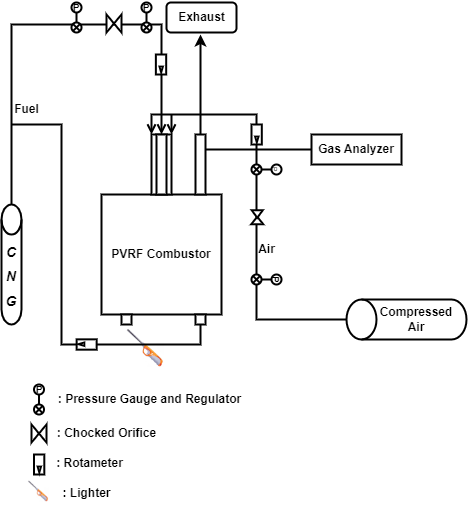
\includegraphics[width=0.5\textwidth]{Chapter4/Images/PVRF.drawio.png}
	\caption{PVRF combustor experimental setup schematic}
	\label{fig1: PVRF}
\end{figure}
\begin{figure}[h]
	\centering
	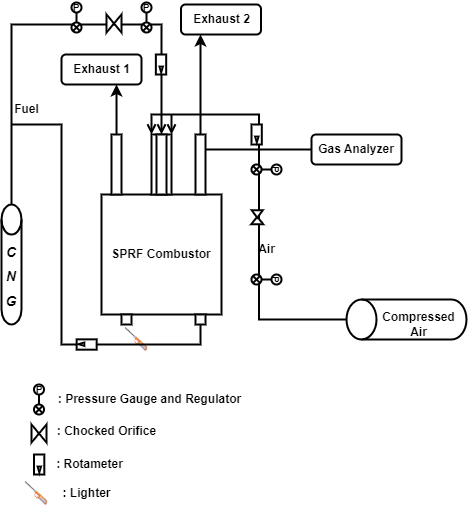
\includegraphics[width=0.5\textwidth]{Chapter4/Images/SPRF.drawio.png}
	\caption{SPRF combustor experimental setup schematic}
	\label{fig2: SPRF}
\end{figure}

Before collecting the experimental data, a settling period of approximately 20 minutes was allocated to the combustor to establish a stable operating condition. This duration ensured that the combustion system reached a fully developed state and maintained consistent performance throughout the subsequent data collection process.

Exhaust gas samples measured by a built-in gas pump was utilized, which drew the gas sample through a probe. The concentration of oxygen in the exhaust gas was measured using a 2-electrode electrochemical sensor based on gas diffusion technology. The pollutant gases emission levels , specifically nitrogen monoxide (NO), and nitrogen dioxide (NO$_2$) and carbon monoxide (CO), were measured using a 3-electrode sensor consisting of a counter, reference, and sensing electrode.

Whenever experimental conditions were changed, such as adjusting the equivalence ratio, it was ensured that the emission readings would be taken after five minutes. This waiting period was essential to ensure precise measurements by allowing the system ample time to adjust and provide consistent emission data.

In order to address experimental variations, each specific setting or condition was repeated three times during the experiments. An estimated uncertainty of approximately $\pm$0.5 ppm was associated with the measurement of NOx emissions, while an uncertainty of approximately $\pm$10$\%$ was associated with the measurement of CO emissions. These uncertainties reflect the inherent variations in the measurement process and instrumentation.


\subsection{Global Imaging}
The reaction zone of methane-air combustion was captured using a mobile camera with a maximum resolution of $3456 \times 4608$ pixels, which corresponds to approximately 15 megapixels. The camera settings used for capturing the images were as follows: a shutter speed of 1/23 s, ISO sensitivity set to 100, and an aperture of f/1.8. The camera was positioned at a fixed distance from the combustor for all the images.

It is important to note that images are not post-processed to change the brightness or contrast. The captured images were raw, without any adjustments or enhancements. This ensures that the captured images accurately represent the observed reaction zone without any artificial alterations. By maintaining consistent camera settings and distance from the combustor, the captured images provide a visual representation of the reaction zone for different equivalence ratios in methane-air combustion.

\subsection{CH$^*$ Chemiluminescene}
Chemiluminescence is a phenomenon observed in combustion processes where the energy released during a chemical reaction is converted into light. This emission of light occurs when excited molecular electronic states return to their ground state by spontaneously emitting photons \cite{NORI2009895, TFVRMGBPJV2011}. The wavelengths of these emitted photons are unique to the species involved in the reaction, and by detecting these wavelengths, valuable information about the presence of specific species in the flame can be obtained.

A selection of commonly observed emitting species in hydrocarbon flames, such as CH$^*$, C$_2^*$, OH$^*$, CO$_2^*$, and H$_2$O$^*$, along with their characteristic wavelengths, is typically provided in Table \ref{Emitting Species}. By analyzing the specific wavelengths at which these species emit light, one can identify their presence and gain insights into the combustion processes taking place within the flame.

\begin{table}[h!]
	\centering
	\begin{tabular}{|c | c |} 
		\hline
		\textbf{Emitting Species} & \textbf{Characteristic Wavelength} \\ [0.5ex] 
		\hline
		OH* & 308.4 nm \\ \hline
        CH* & 431.5 nm \\ \hline
        C* & 436-563 nm \\ \hline
        $CO_2$* & Broadband from 340-650 nm \\ \hline
        Incandescent soot & Continuous (function of temperature) \\ \hline
	\end{tabular}
	\caption[Emitting species found in a hydrocarbon flame and their characteristic wavelength]{Emitting species found in a hydrocarbon flame and their characteristic wavelength (Data is taken from \cite{KARNANI20132275}).}
	\label{Emitting Species}
\end{table}

\subsection{Gas Analyzer}
In this study, the flue gas analysis was performed using the MRU OPTIMA7 multigas handheld gas analyzer. This analyzer have a built-in gas pump that draw sample of flue gases through a probe from combustor. A built-in filter processed the sample by passing it through condensate seperator to ensure it is clean and dry. Finally, electrochemical sensors analyze the gas sample.

The MRU OPTIMA7 gas analyzer is capable of measuring various parameters of the flue gases, such as oxygen (O2) concentration, carbon monoxide (CO) concentration, nitrogen oxide (NOx) levels, sulfur dioxide (SO2) levels, and other relevant combustion gases. The electrochemical sensors in the analyzer provide accurate and real-time measurements of these gas concentrations, allowing for the analysis of flue gas composition and emissions.

\subsection{Combustor Design and Ignition Process}
Figure \ref{PVRF-geometry} and \ref{SPRF-geometry} shows schematic and photograph of the PVRF and SPRF combustor. The dimensions of combustor is 80 $\times$ 80 $\times$ 40 (in mm). The air and fuel injection take place co-axially at the top and along the centerline of the combustor in non-premixed mode. In premixed mode, fuel tube is removed and at far upstream point, air and fuel are mixed properly and then injected in combustion chamber. In the PVRF combustor, the air injection port (with a diameter of 10 mm) is positioned 40 mm from the right wall, while the fuel injection port (with a diameter of 2 mm) is coaxial with the air injection port. The air and exit ports are located at a distance of 25 mm from their respective centres, while the exit port is positioned at a distance of 15 mm from the right wall of the combustor.

In the SPRF combustor, an additional exit port is added at a distance of 25 mm from the air port and 15 mm from the left wall. Both exit ports are symmetrically placed along the air port axis. The ignition port, or pilot burner, is located at the bottom right of the combustor, 15 mm from the right wall. An external igniter is used to initiate the combustion and is subsequently closed by a insulated plug to avoid any secondary flow. The ignition port has a diameter of 10 mm. The pilot fuel port, used to supply the fuel during initial combustion stage, is situated at the bottom right, 15 mm from the left wall, and has a diameter of 5 mm.

\begin{figure}[h]
	\centering
	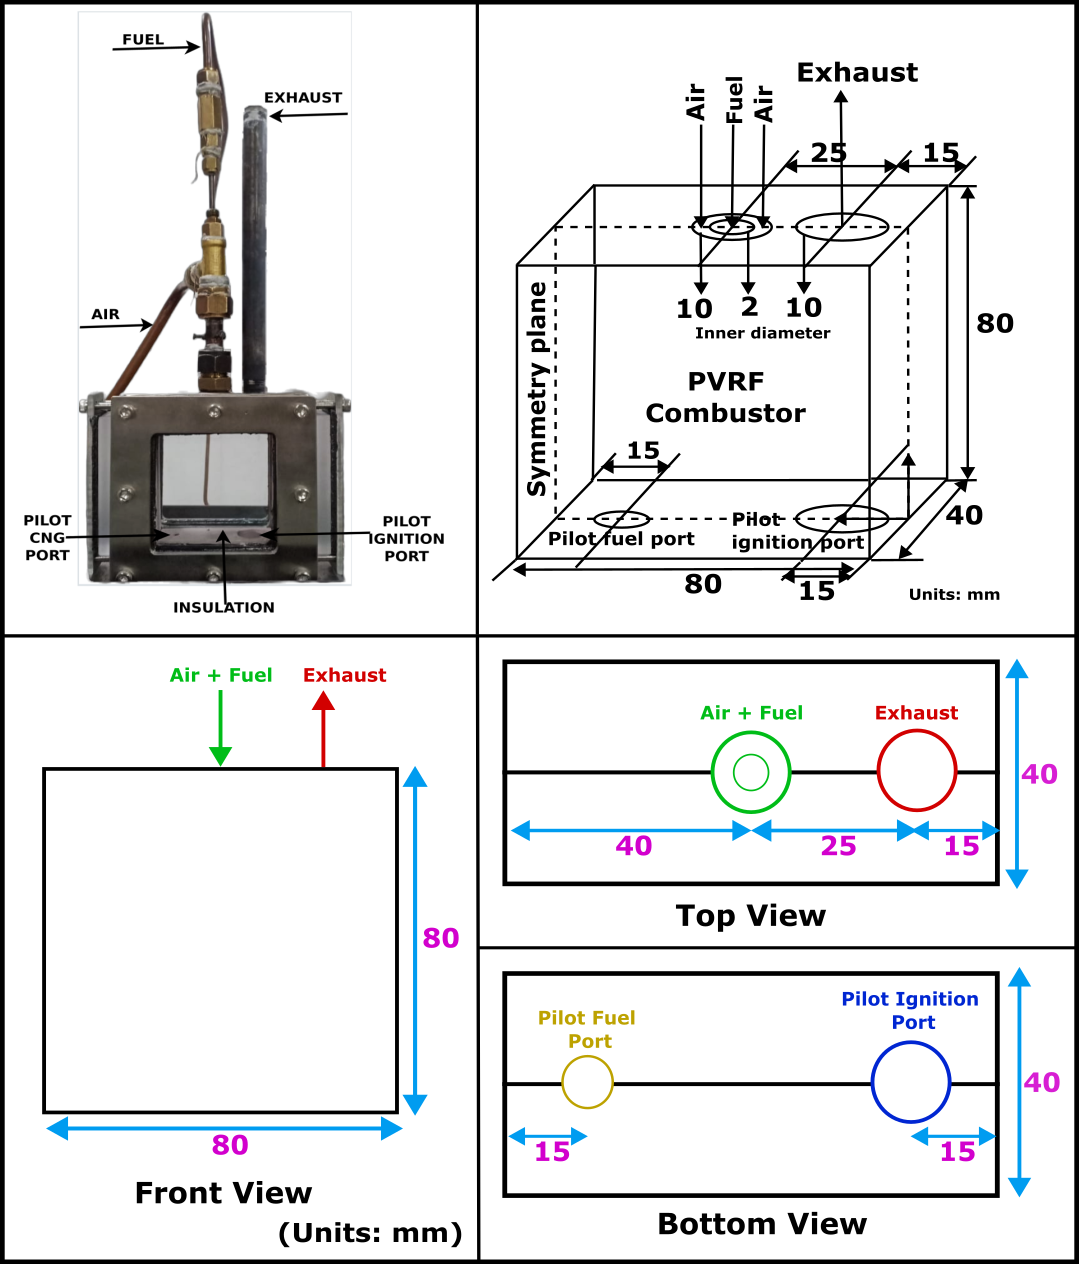
\includegraphics[width=0.95\textwidth]{Chapter4/Images/PVRF_Lab.png}
	\caption{PVRF combustor schematic and photograph}
	\label{PVRF-geometry}
\end{figure}
\begin{figure}[h]
	\centering
	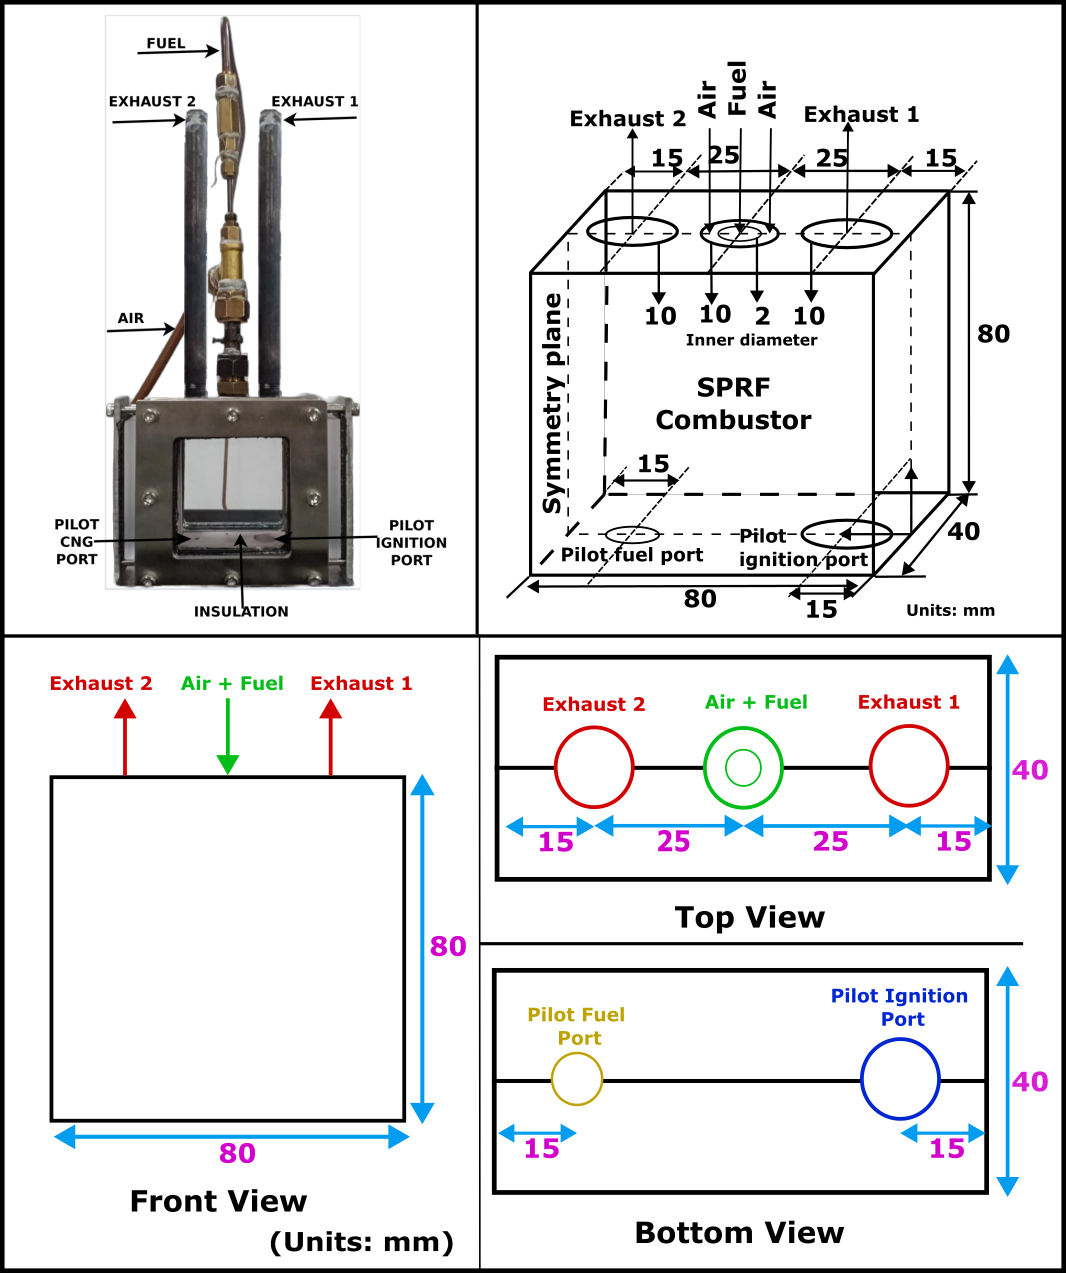
\includegraphics[width=0.95\textwidth]{Chapter4/Images/SPRF_Lab.png}
	\caption{SPRF combustor schematic and photograph}
	\label{SPRF-geometry}
\end{figure}
